\section{Effective mass equation}
\thm{Effective mass equation}{
	\begin{align}
		\psi(\vec{r}, t) &= \sum_{\vec{k}}^{}c_{\vec{k}}(t)\psi_{n, \vec{k}}(\vec{r}) \nonumber \\
		&= \sum_{\vec{k}}^{}c_{\vec{k}}(t)u_{n, \vec{k}}(\vec{r})e^{i\vec{k}\cdot\vec{r}} \label{eqn:eff_mass_above}
	\end{align}
	We will restrict the coeficcients $c_{\vec{k}}(t)$ to values around $\vec(k)_0$, where $\vec(k)_0$ is located a a band extremum. We get a visualization like
	\begin{center}
		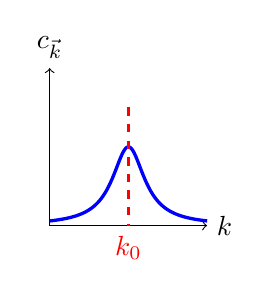
\begin{tikzpicture}
			\draw[->, black]	(0, 0) to (2, 0) node[right]{$k$};
			\draw[->, black]	(0, 0) to (0, 2) node[above]{$c_{\vec{k}}$};

			\draw[blue, very thick]	plot[samples=200, domain=-4:4] ({\x/4 + 1}, {1/(1 + \x*\x)});

			\draw[red, dashed, thick] 	(1, 1.5) to (1, 0) node[below]{$k_0$};
		\end{tikzpicture}
	\end{center}
	Because they are sharply peaked we can write equation \ref{eqn:eff_mass_above} as
	\begin{align}
		\psi(\vec{r}, t) &= \sum_{\vec{k}}^{}c_{\vec{k}}(t)u_{n, \vec{k}_0}(\vec{r})e^{i\vec{k}\cdot\vec{r}} \nonumber \\
		&= \sum_{\vec{k}}^{}c_{\vec{k}}(t)u_{n, \vec{k}_0}(\vec{r})e^{i\vec{k}\cdot\vec{r}}e^{i\vec{k}_0\cdot\vec{r}}e^{-i\vec{k}_0\cdot\vec{r}} \nonumber \\
		&= \sum_{\vec{k}}^{}c_{\vec{k}}(t)e^{i(\vec{k}-\vec{k}_0)\cdot\vec{r}}\psi_{n, \vec{k}_0}(\vec{r}) \nonumber \\
		&= \psi_{n, \vec{k}_0}(\vec{r})\sum_{\vec{k}}^{}c_{\vec{k}}(t)e^{i(\vec{k}-\vec{k}_0)\cdot\vec{r}} \label{eqn:new_psi}
	\end{align}
	The function $\sum_{\vec{k}}^{}c_{\vec{k}}(t)e^{i(\vec{k}-\vec{k}_0)\cdot\vec{r}}$ will oscillate if $\vec{k}$ is far away from $\vec{k}_0$, which cannot happen. Therefore this function varies slowly in time. This funtion is called the \textbf{envelope wave function}:
	\begin{equation}
		F(\vec{r}, t) = \sum_{\vec{k}}^{}c_{\vec{k}}(t)e^{i(\vec{k}-\vec{k}_0)\cdot\vec{r}}
	\end{equation}
	Yet again, we have constructed some kind of wave packet. In particular, it turns out that if we restrict the coefficients around the values $k_0$ (with some deviation $\Delta k$, $\Delta k << \frac{2\pi}{a}$). This implies that the uncertainty of the position $\Delta x >> a$. \\
	This is a result from the fourier analyis and wave-packets that give a relation $\Delta x \Delta k > 1$, it is the same relation that gives rise to the Heisenberg uncertainty principle. \\ \newline
	How does this description of the wavefunction behave when the operator $\hat{E}(-i\vec{\nabla})$ acts on it? We perform the same principle as in section \ref{sec:eff_mass_th}
	\begin{align}
		\hat{E}(-i\vec{\nabla})\psi(\vec{r}, t) &= \hat{E}(-i\vec{\nabla})\left[\psi_{n, \vec{k}_0}(\vec{r})F(\vec{r}, t)\right] \\
		&= \sum_m^{}E_me^{\vec{R}_m\cdot\vec{\nabla}}\left[\psi_{n, \vec{k}_0}(\vec{r})F(\vec{r}, t)\right] \\
		&= \sum_m^{}E_m\psi_{n, \vec{k}_0}(\vec{r} + \vec{R}_m)F(\vec{r} + \vec{R}_m, t) \\
		\text{using Bloch} \qquad &= \sum_m^{}E_me^{i\vec{R}_m\cdot\vec{k}_0}\psi_{n, \vec{k}_0}(\vec{r})e^{\vec{R}_m\cdot\vec{\nabla}}F(\vec{r}, t) \\
		&= \sum_m^{}E_m\psi_{n, \vec{k}_0}(\vec{r})e^{i\vec{R}_m\cdot(\vec{k}_0 - i\vec{\nabla})}F(\vec{r}, t) \\
		&= \psi_{n, \vec{k}_0}(\vec{r})\sum_m^{}E_me^{i\vec{R}_m\cdot(\vec{k}_0 - i\vec{\nabla})}F(\vec{r}, t)
	\end{align}
	And this is nothing else as
	\begin{equation}
		\psi_{n, \vec{k}_0}(\vec{r})\hat{E}(\vec{k}_0 - i\vec{\nabla})F(\vec{r}, t) \label{eqn:make_use}
	\end{equation} \\ \newline
	As a result, using the effective mass theorem we can become a more general description (i.e. the effective mass equation) by making use of equation \ref{eqn:new_psi} and equation \ref{eqn:make_use}:
	\begin{equation}
		i\hbar\frac{\delta F}{\delta t} = \left[\hat{E}(\vec{k}_0 - i\vec{\nabla}) + V_{ext}\right]F(\vec{r}, t)
	\end{equation}
}
How can we use the effective mass equation? Suppose we look at a CB minimum located at $\vec{k}_0$, not located at the $\Gamma$-point. We can than say that because we are at a minium, we can write
\begin{equation}
	E_n(\vec{k}) = E_n(\vec{k}_0) + \frac{1}{2}\sum_{i, j}^{} \left\frac{\delta^2E_n(\vec{k})}{\delta k_i \delta k_j}\right|_{\vec{k} = \vec{k}_0}(k_i -k_{i, 0})(k_j - k_{j, 0})
\end{equation}
Then the effecive mass eqution becomes:
\begin{align}
	i\hbar\frac{\delta F}{\delta t} &= \left[\hat{E}(\vec{k}_0 - i\vec{\nabla}) + V_{ext}\right]F(\vec{r}, t) \\
	&\text{where} \quad \hat{E}(\vec{k}_0 - i\vec{\nabla}) = E_n(\vec{k}_0) - \frac{1}{2}\sum_{i, j}^{} \left\frac{\delta^2E_n(\vec{k})}{\delta k_i \delta k_j}\right|_{\vec{k} = \vec{k}_0}\frac{\delta}{\delta r_i} \frac{\delta}{\delta r_j} \\
	\text{using equation \ref{eqn:eff_mass_tensor}}\quad \Rightarrow \quad i\hbar\frac{\delta F}{\delta t} &= \left[\hat{E}_n(\vec{k}_0) - \frac{\hbar^2}{2}\sum_{i, j}^{}\left[m^{*}_{i, j}\right]^{-1}\frac{\delta}{\delta r_i} \frac{\delta}{\delta r_j} + V_{ext}\right]F
\end{align}
\ex{Using the effective mass equation - 1D}{
	Consider a CB minimum at $k = 0$. Then, the conduction band is described by:
	\begin{equation*}
		E_{CB}(k) = E_{CB} + \frac{\hbar^2k^2}{2m^*} \qquad \text{with } m^* > 0
	\end{equation*}
	Then, we can find the envelope wave function as
	\begin{equation*}
		i\hbar\frac{\delta F}{\delta t} = \left[E_{CB} - \frac{\hbar^2}{2m^*}\frac{d^2}{dx^2} + V_{ext}\right]F
	\end{equation*}
	Say we take $V_{ext} = 0$, then (after filling in $F(x, t) = \psi(x)e^{-iEt/\hbar}$) we get:
	\begin{equation*}
		-\frac{\hbar^2}{2m^*}\frac{d^2}{dx^2}\psi(x) = (E - E_{CB})\psi(x)
	\end{equation*}
	This is just a normal time independent Schrödinger equation.
}
Remember that earlier was said that when working with acceptors and donors, the energy levels of these acceptors and donors, first of all, were in the energy gap, but also that they had a hydrogen-like energy spectrum. From that spectrum, it is possible to derive the ionization energy for the energy levels of the acceptors and donors.
\ex{E-spectrum of donor impurities in GaAs (III - V)}{
	We will replace Ga by Si. Then wat is the $V_{ext}$ introduced by Si? Well what we want to know is the folowing
	\begin{align*}
		V_{ext}(\vec{r}) &= V_{Si}(\vec{r}) - V_{Ga}(\vec{r}) \\
		&= -\frac{(Z_{Ga} + 1)e^2}{4\pi\epsilon\abs{\vec{r}}} + \frac{Z_{Ga}e^2}{4\pi\epsilon\abs{\vec{r}}} \\
		&= -\frac{e^2}{4\pi\epsilon\abs{\vec{r}}}
	\end{align*}
	We know that the energy is given by:
	\begin{equation*}
		E(\vec{k}) = E_c + \frac{\hbar^2k^2}{2m^*}
	\end{equation*}
	Then the effective mass equation becomes:
	\begin{align*}
		i\hbar\frac{\delta F}{\delta t} &= \left[E_c - \frac{\hbar^2}{2m^*}\nabla^2 - \frac{e^2}{4\pi\epsilon\abs{\vec{r}}}\right]F(\vec{r}, t) \\
		&\text{with} \qquad F(\vec{r}, t) = \psi(\vec{r})e^{-i/\hbar Et} \\
		\left[- \frac{\hbar^2}{2m^*}\nabla^2 - \frac{e^2}{4\pi\epsilon\abs{\vec{r}}}\right]\psi(\vec{r}) = (E - E_c)\psi(\vec{r})
	\end{align*}
	This is just the Schrödinger equation for a hydrogen atom with one electron, instead now with an effective mass $m^*$. Particulary, we are looking for the \textbf{bound states}.
	For hydrogen we know then that $E - E_c$ must be given by
	\begin{equation*}
		E - E_c = -\frac{e^4m^*}{2n^2(4\pi\epsilon\hbar)^2} \qquad \text{with } n = 1, 2, \dots
	\end{equation*}
	Now we have degeneracies and an ionization energy. Once this energy level is passed, electrons can freely move in the conduction band. The result is given in this figure:
	\begin{center}
		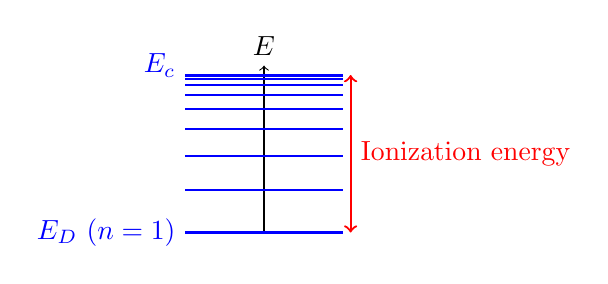
\begin{tikzpicture}
			\draw[->, black]	(0, -0.12) to (0, 2) node[above]{$E$};

			\foreach \y in {1,...,10} {
				\draw[blue, thick]	plot[samples=200, domain=-1:1] (\x, {1.88-\y*\y*\y/500});
			}

			\draw[<->, red, thick]		(1.1, -0.12) to node[right]{Ionization energy} (1.1, 1.88);

			\draw[blue]		(-1, -0.12) node[left]{$E_D$ $(n = 1)$};
			\draw[blue]		(-1, 2) node[left]{$E_c$};
		\end{tikzpicture}
	\end{center}
}
\ex{E-spectrum of acceptor impurities in Si}{
	Now, we will replace Si by an acceptor.
	1h01
}
